\section{Methods}

\subsection{Notation}
Before we present our new SOM learning algorithm, we introduce the notation 
and terminology we are using throughout the present work. We borrow the
notation from a previous work~\citep{rougier:2011}. 
A neural map is defined to be the projection from a manifold
$\Omega \subset \mathbb{R}^d$ onto a set $\mathcal{N}$ of $n$ {\em neuron}s
$\Phi : \Omega \rightarrow \mathcal{N}$.
Each neuron $i$ is associated with a code word $\mathbf{w}_i \in
\mathbb{R}^d$, all of which establish the set 
$\mathcal{W} = \{\mathbf{w}_i, i \in \mathcal{N}\}$ that is referred as the code book. The mapping from $\Omega$ to
$\mathcal{N}$ is a closest-neighbor winner-take-all rule such that any vector
$\mathbf{v} \in \Omega$ is mapped to a neuron $i$ with the code
$\mathbf{w}_\mathbf{v}$ being closest to the current input vector
$\mathbf{v}$,
\begin{equation}
\Phi : \mathbf{v} \mapsto argmin_{i \in \mathcal{N}} (\lVert \mathbf{v} -
\mathbf{w}_i \rVert).
\label{eq:psi}
\end{equation}
The neuron $\mathbf{w}_\mathbf{v}$ is named the best matching unit (BMU) and
the set $C_i = \{x \in \Omega | \Phi(x) = \mathbf{w}_i \}$ defines the {\em
  receptive field} of neuron $i$.


\subsection{Spatial distribution} % \& Centroidal Voronoi Tesselation}
\label{sec:spatial_dist}

The SOM space is usually defined as a two-dimensional manifold where nodes are
arranged in a regular lattice (rectangular or hexagonal). Here, we follow a 
different approach and instead of the regular lattice we place the neurons
randomly by sampling a specific spectral distribution. More specifically, we
assign neurons positions by drawing samples from a Blue noise distribution. 
\citet{Zhou:2012}. have shown that the spectral distribution
property of noise patterns is often described in terms of the Fourier spectrum
color. For instance, white noise corresponds to a flat spectrum with signal's
energy equally distributed to all frequency bands. On the other hand, blue 
noise has weak low-frequency energy and strong high-frequency energy. This
means that the signal stores its energy mostly on the high-frequency
components introducing a form of data compression \gid{[CITATION REQ.]}.
Another interesting, and useful in this work, property of blue noise is that 
the positions of neurons drawn by a blue noise distribution are 
evenly spread without any apparent structure (see figure~\ref{fig:sampling}
for a comparison of spatial distributions).
%%
\begin{figure}[htbp]
  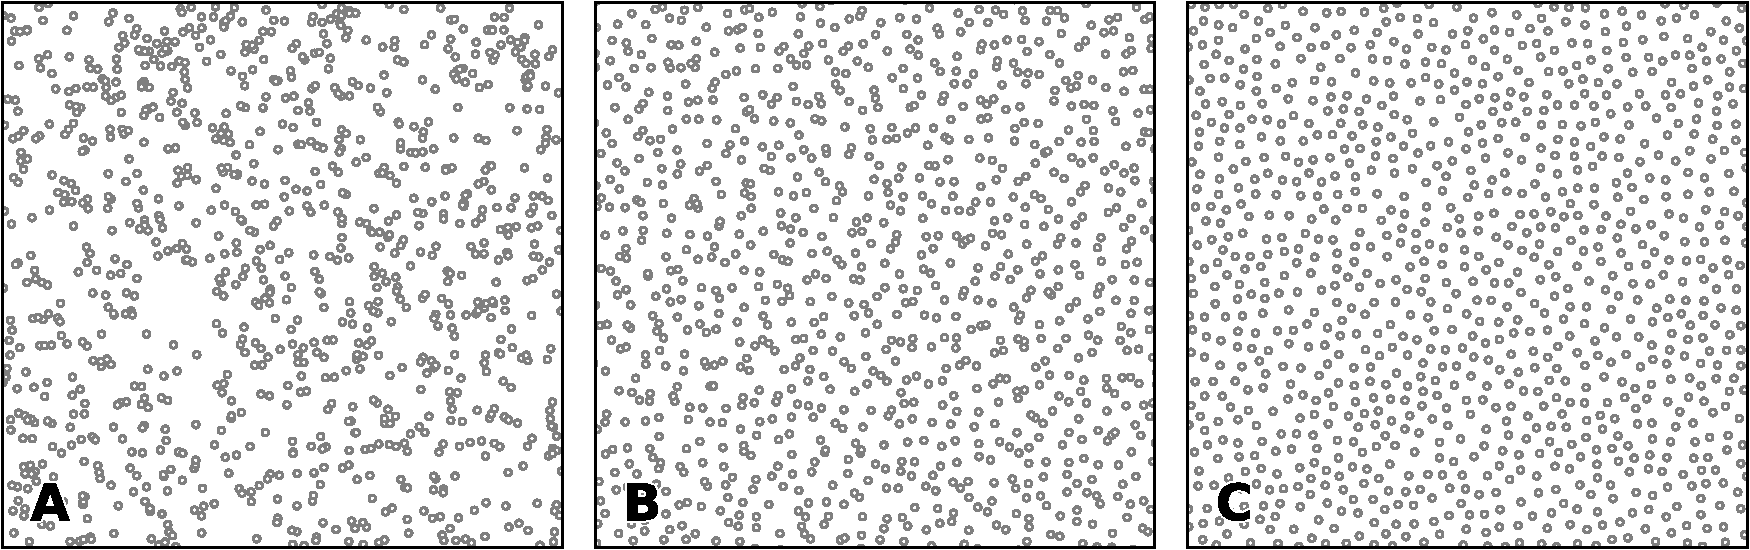
\includegraphics[width=\textwidth]{figures/blue-noise.pdf}
  \caption{\textbf{Spatial distributions.}
    \textbf{\textsf{A.}} Uniform sampling (n=1000) corresponding to white noise.
    \textbf{\textsf{B.}} Regular grid (n=32$\times$32) + jitter (2.5\%).
    \textbf{\textsf{C.}} Poisson disc sampling (n=988) corresponding to blue noise.}
  \label{fig:sampling}
\end{figure}
%%

Blue noise distributions exist for many years. They have being used in the
field of computer graphics for Poisson disk sampling, dart throwing, relaxation,
tiling, and other applications~\citep{Lagae:2008}. One of the fastest
and easiest to implement method for generating blue noise samples is the 
fast Poisson disk sampling. This method introduced by~\citep{Bridson:2007} 
and performs on arbitrary dimensions at linear time ($\mathcal{O}(n)$).
In this work, we imply this method for placing neurons over a normalized 
region of $[0,1]\times[0,1]$. Such Poisson disk sampling guarantees that 
samples are no closer to each other than a specified minimum radius. This
initial placement is further refined by applying a LLoyd relaxation~\citep{Lloyd:1982}
scheme for $10$ iterations to achieve a quasi centroidal Voronoi tesselation.

\subsection{Topology}
\label{sec:topo}

Consider a set $P$ of $n$ points on a finite region of $[0, 1] \times [0, 1]$. 
The steps we follow to determine the topology of the SOM are:
First, we compute the Euclidean distance matrix ${\bf E} \in \mathbb{R}^{n\times n}$,
where $e_{ij} = \lVert p_i - p_j \rVert$ and $i, j=1, \ldots, n$. Subsequently 
we define a connectivity matrix ${\bf G}_m$ with elements $g_{ij} = 1$ if 
$p_j$ belongs to the $m$ closest points to $p_i$ and $g_{ij} = 0$ otherwise.
This definition implies that the matrix ${\bf G}_m$ carries information about
connected neurons within a predetermined vicinity. Once we compute matrix
${\bf G_m}$, which essentially represents a graph, we compute the shortest
path between each pair of nodes on the graph and we store them into a new
matrix called ${\bf D}_m$. Note that lengths are measured in number of nodes
(hops) required to reach two nodes such that the two corresponding Euclidean
points (represented by the nodes) may have a graph distance as illustrated in 
figure \ref{fig:topology}. 
\gid{This matrix
distance is then normalized by dividing it by the maximum distance between two
nodes. NOT VERY CLEAR}.
In the degenerative case where two nodes are not connected on the graph, we
resample from a spatial distribution until all nodes have degree greater than 
one (are connected at least with one other node \gid{IS THIS CORRECT?}).
%%
\begin{figure}
  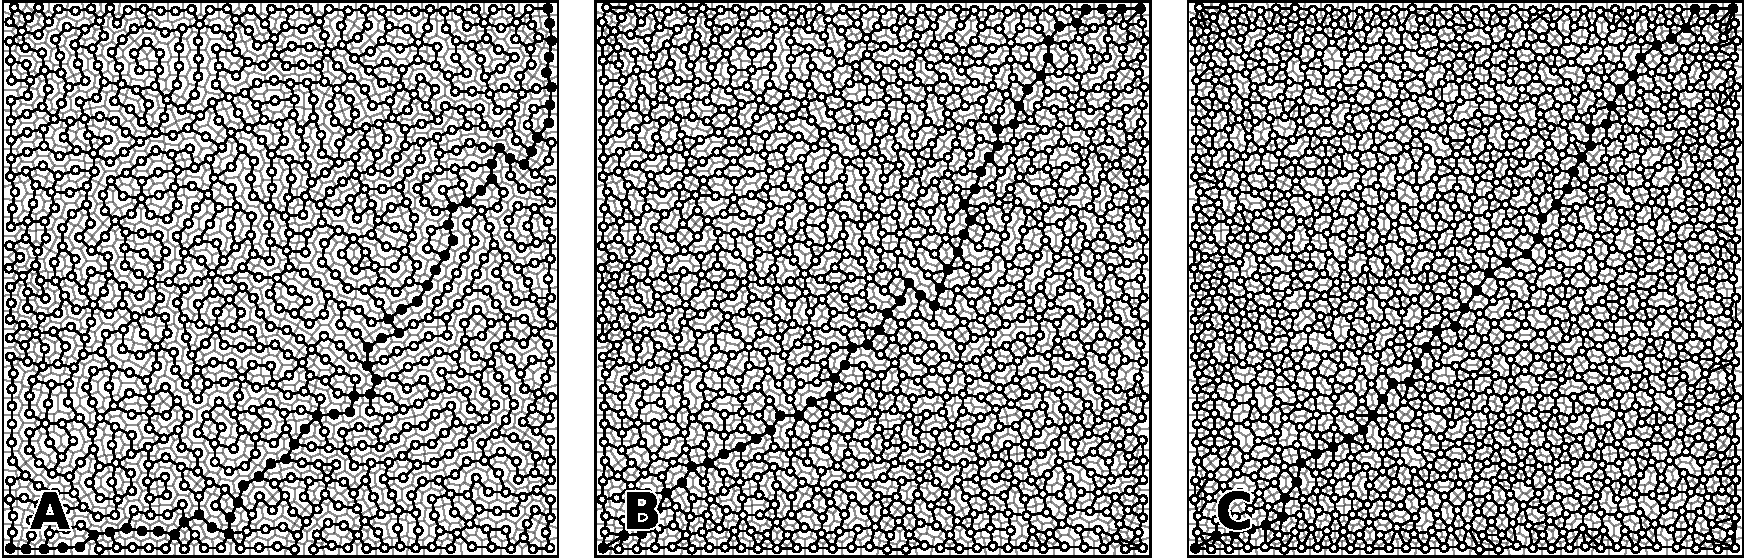
\includegraphics[width=\columnwidth]{figures/distances.pdf}
  \caption{\textbf{Influence of the number of neighbours on the graph
    distance.} The same initial set of 1003 neurons has been equiped with
    2-nearest neighbors, 3 nearest neighbors and 4-nearest neighbors induced
    topology (panels \textbf{A}, \textbf{B} and \textbf{C} respectively). A
    sample path from the the lower-left neuron to the upper-right neuron has
    been highlighted with a thick line (with respective lengths of 59, 50 and
    46 nodes).}
  \label{fig:topology}
\end{figure}


\subsection{Learning}

The learning algorithm we propose in this work relies on the standard SOM 
algorithm~\citep{Kohonen:1982}. Once we have define the topology of the map
following the steps we described in paragraph~\ref{sec:topo}, we can start 
the learning process. Learning is iterative and starts at a time $t_0=0$ and
runs until some predetermined final time step, $t_f \in \mathbb{N}^+$, has been 
reached. At every iteration input vectors $\mathbf{v} \in \Omega$ are 
sequentially given to the
map with respect to the probability density function $f$ \gid{Where is defined?}.
For each vector $\mathbf{v}$ at time $t$, a winner neuron with index 
$s \in \mathcal{N}$ is determined according to equation (\ref{eq:psi}). This
means that at time $t$ neuron $s$ is closer to the input vector ${\bf v}$, in
the sense of Euclidean distance, than any other neuron. 
Once the winner neuron has been identified all codes $\mathbf{w}_{i}$ from the
current code book are shifted towards $\mathbf{v}$ according to
\begin{align}
\label{eq:som-learning}
    \Delta\mathbf{w}_{i} &= \varepsilon(t)~h(t,i,s;\sigma)~(\mathbf{v} - \mathbf{w}_i), 
\end{align}
where $s$ is the index of the winner neuron, $i$ is the index of code words
in the code book and $t$ is the current time step. $h_\sigma(t,i,j;\sigma)$ is
a neighborhood function of the form
\begin{equation}
  h(t,i,j; \sigma) = \exp\Big(-\frac{{d_{ij}}^2}{\sigma(t)^2}\Big)
  \label{eq:som-neighborhood}
\end{equation}
where $\varepsilon: \mathbb{R} \rightarrow \mathbb{R}$ is the learning rate
time-dependent function given by
$\varepsilon(t) = \varepsilon_i\left(\frac{\varepsilon_f}{\varepsilon_i}\right)^{t/t_f}$,
where $\varepsilon_i$ and $\varepsilon_f$ are the initial and final
learning rates, respectively.
$\sigma: \mathbb{R} \rightarrow \mathbb{R}$ is determines the width of the 
neighborhood function~\eqref{eq:som-neighborhood} and it is reads
$\sigma(t) = \sigma_i\left(\frac{\sigma_f}{\sigma_i}\right)^{t/t_f}$,
where $\sigma_i$ and $\sigma_f$ are the initial and final neighborhood widths,
respectively. We usually assume $\sigma_f \ll \sigma_i$ and 
$\varepsilon_f \ll \varepsilon_i$. The entire learning procedure is summarized
by Algorithm~\ref{algo:vsom}. 


%%
\begin{algorithm}[!htpb]
	\begin{algorithmic}
    	\Require $\mathcal{S}$, $\mathcal{N}$, $t_f$, $dt$, $\varepsilon_i$, $\varepsilon_f$, $\sigma_i$, $\sigma_f$
        \Ensure ${\bf W}$
        \If {\text{Blue noise is True}}
        	\State Compute blue noise distribution $\mathcal{B}$
        	\State Compute $e_{ij} = || p_i - p_j ||$		\Comment{Euclidean pair distances matrix}
        	\State Construct matrix ${\bf G}_m$			\Comment{Connectivity matrix}
        	\State Compute matrix ${\bf D}_m$			\Comment{Shortest paths between nodes}
        	\State Place neurons positions on points sampled from $\mathcal{B}$
        \Else
        	\State Discretize grid $[0, 1]\times[0, 1]$ and place neurons on its nodes
        \EndIf
        
        \State $w_s \gets \varnothing$, ${\bf W} \sim \mathcal{U}(0, 1)$	\Comment{Initialize winner unit and code book}
                 
        \For{$t \gets 0, \ldots, t_f$}
        	\State ${\bf v} \gets \bf{s}_t $	\Comment{${\bf s}_t \in \mathcal{S}$}
        	\State $s \gets argmin_{i \in \mathcal{N}} (\lVert \mathbf{v} - \mathbf{w}_i \rVert)$
        	\State $\varepsilon(t) = \varepsilon_i\left(\frac{\varepsilon_f}{\varepsilon_i}\right)^{t/t_f}$
        	\State $\sigma(t) = \sigma_i\left(\frac{\sigma_f}{\sigma_i}\right)^{t/t_f}$
        	\State $h(t,i,j; \sigma) = \exp\Big(-\frac{{d_{ij}}^2}{\sigma(t)^2}\Big)$
        	\State ${\bf w}_i^{\text{new}} = {\bf w}_i^{\text{old}} + \varepsilon(t) \odot h(t,i,s;\sigma) \odot (\mathbf{v} - \mathbf{w}_i^{\text{old}})$
        \EndFor
	\end{algorithmic}
\caption{Voronoi Self-organizing Map (vSOM). $\mathcal{N}$ is neurons index set,
$\mathcal{I}$ is the input dataset, $t_f$ is the simulation time (or the number of input samples).
$\varepsilon_i$ and $\varepsilon_f$ are the initial and final learning rates,
respectively. $\sigma_i$ and $\sigma_f$ are the initial and final neighborhood
widths. $\odot$ is the Hadamard product.}
\label{algo:vsom}
\end{algorithm}
%%



\subsection{Simulation Details}

We conduct all the experiments using the parameters provided by
Table~\ref{table:parameters}. In all the experiments the input space is
the Cartesian product $[0, 1] \times [0, 1]$ and neurons positions drawn from
a blue noise distribution using the fast Poisson disk sampling
algorithm~\citep{Bridson:2007} (see paragraph~\ref{sec:spatial_dist} for more details). 
The source code of the proposed algorithm is written in the Python programming
language (SciPy~\citep{Jones:2001}, Matplotlib~\citep{Hunter:2007}
and NumPy~\citep{Walt:2011}). Sources are available at 
\href{https://github.com/rougier/VSOM}{github.com/rougier/VSOM}.
All the experiments run on a [] machine equipped with []$\,\mathrm{GB}$ physical
memory and [] operating system. 
%%
\begin{table}[!ht]
  \begin{center}
    \begin{tabular}{ll}
        \textbf{Parameter} & \textbf{Value} \\
        \hline
        Number of epochs      ($t_f$)           & 25000\\
        Learning rate initial ($\varepsilon_i$) & 0.50\\
        Learning rate final   ($\varepsilon_f$) & 0.01\\
        Sigma initial         ($\sigma_i$)      & 0.50\\
        Sigma final           ($\sigma_f$)      & 0.01\\
    \end{tabular}
      \caption{\textbf{Default parameters} Unless specified otherwise, these are
        the parameters used in all the simulations.}
      \label{table:parameters}
  \end{center}
\end{table}


%% Considering a set of $n$ points $P = \{P_i\}_{i \in [1,n]}$ on a finite domain
%% $D \in \mathbb{R}^2$, the Voronoi tesselation $V(P) = \{V_i\}_{i \in [1,n]}$ of
%% $P$ is defined as:
%% %
%% \begin{equation}
%%   \forall i \in [1,n], V_i = \{x \in D \mid
%%   \lVert x - P_i \rVert \leq \lVert x - P_j \rVert, \forall j \neq i\}
%% \end{equation}
%% %
%% Reciprocally, the (unique) Delaunay triangulation $T(P) = \{T_i\}_{i \in
%%   [1,n]}$ of $P$ is the dual graph of the Voronoi diagram and defined such that
%% no point in $P$ is inside the circumcircle of any triangles in $T(P)$. The
%% centers of the circumcircles are equivalent to the Voronoi diagram, i.e. a
%% partition of $D$ into Voronoi cells. For each of the cell $V_i$, we can compute
%% its centroid $C_i$ which is the center of mass of the cell. A Voronoi
%% tesselation is said to be centroidal when we have $\forall i \in [1,n], C_i =
%% P_i$ (see figure~\ref{fig:CVT}).\\

%% For an arbitrary set of points, there is no guarantee that the corresponding
%% Voronoi tesselation is centroidal but different methods can be used to
%% generate a centroidal tesselation from an arbitrary set of points. One of the
%% most straightforward and iterative methods is the Lloyd relaxation scheme
%% \citep{Lloyd:1982}:
%% \begin{enumerate}
%%   \item The Voronoi diagram of the $n$ points is computed
%%   \item The centroid of each of the $n$ Voronoi cell is computed.
%%   \item Each point is moved to the corresponding centroid of its Voronoi cell
%%   \item The method terminates if criterion is met (see below), else go to 1
%% \end{enumerate}
%% The algorithm finishes when the maximum distance between points and centroids
%% is less than a given threshold as illustrated in figure~\ref{fig:CVT}. It is
%% to be noted that because of numerical imprecisions, there is no guarantee that
%% an arbitrary small threshold can be reached.


%% \begin{figure}[htbp]
%%   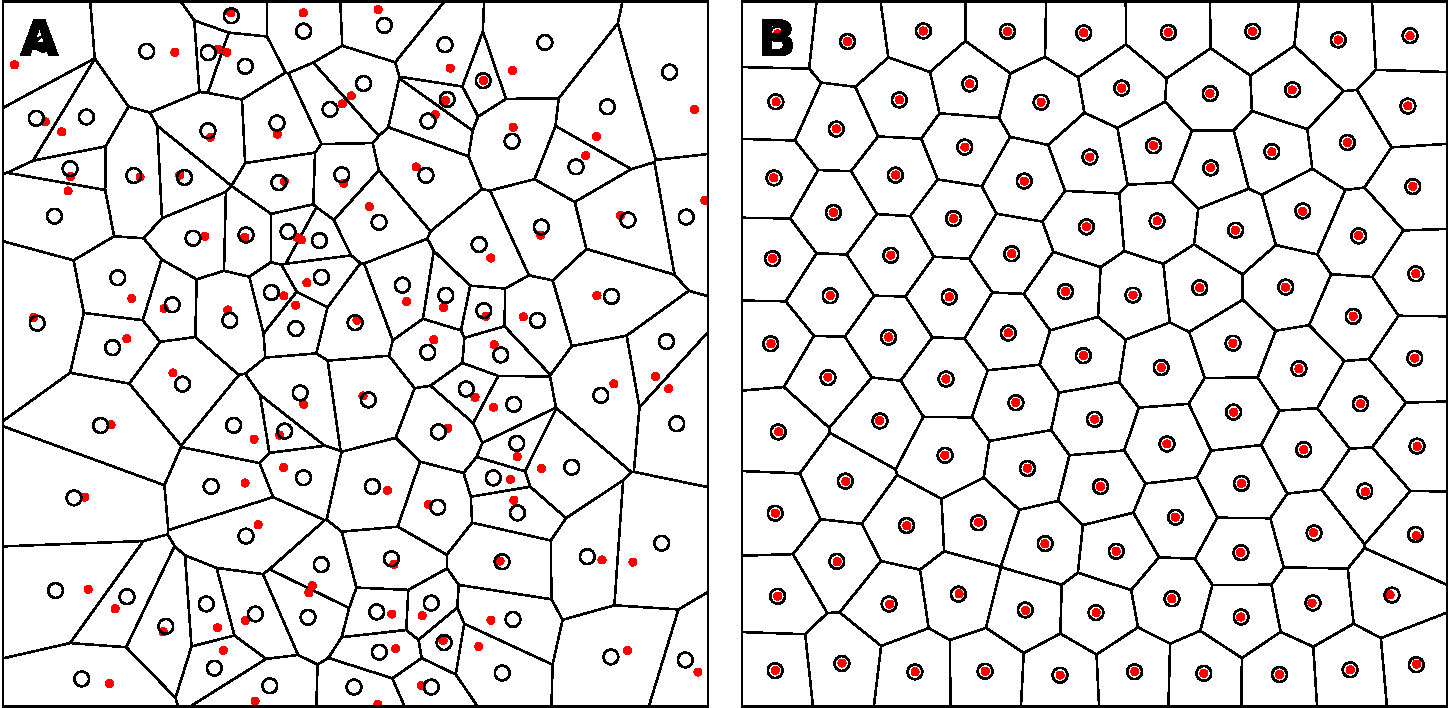
\includegraphics[width=\textwidth]{figures/CVT.pdf}
%%   \caption{\textbf{Centroidal Voronoi Tesselation.}  \textbf{\textsf{A.}}
%%     Voronoi diagram of a uniform distribution (n=100) where red dots represent
%%     the uniform distribution and white circles represent the centroids of each
%%     Voronoi cell. \textbf{\textsf{B.}} Centroidal Voronoi diagram where the
%%     point distribution matches the centroid distribution which constitutes a
%%     blue noise distribution (i.e. {\em a distribution that is roughly uniformly
%%       random with no preferred inter-point directions or distances} according
%%     to the definition of \citep{Ebeida:2014}). This figure has been obtained
%%     from the initial distribution on the left after 50 iterations of the Lloyd
%%     relaxation algorithm. }
%%   \label{fig:CVT}
%% \end{figure}
%
